% boosting.tex
% Jeremy Barnes, 29/8/1999
% $Id$

% The chapter of my thesis on Boosting

\chapter{Boosting and similar algorithms}

The name ``Boosting'' is applied to many different machine learning
algorithms, which combine many weak hypotheses to form a ``strong''
hypothesis that significantly outperforms them.

We first describe the classic algorithm \emph{AdaBoost}.  A full
description is given, along with some examples of its performance and
a discussion of why it performs so well.  We also give a formal
definition of what we mean by the term ``boosting''.

A useful viewpoint of the boosting algorithm as an optimisation via
gradient descent in a cost space is then considered.  A result from
Mason et al. \cite{Mason99} is derived which shows that boosting is
indeed performing gradient descent.

We then consider \emph{normed boosting algorithms} where the
weights of the hypotheses are constrained by some norm.  Several
properties of these algorithms which are different from those of
unconstrained boosting algorithms are discussed.

We then turn to questions of the performance of boosted algorithms; in
particular guarantees on the training and generalisation error.
Several results are presented.

Finally, we motivate the $p$-boosting algorithm by considering the
problem of overfitting in boosting.  Both practical and theoretical
explanations for this phenomenon are given.


\section{The original boosting algorithm: AdaBoost}

We first describe the AdaBoost algorithm, first published by Freund
and Scahpire \cite{Freund96}.  In essence, this algorithm
``bootstraps'' itself onto another learning algorithm (the \emph{weak
learning algorithm}) and improves the performance by producing a
linear combination of weak learning hypotheses.

AdaBoost performs \emph{very} well; its combined hypotheses generally
perform significantly better than \emph{any} non-boosted algorithm.
This is particularly true for reliable (low-noise) data.  Even
the simplest of weak algorithms, when ``boosted'', will usually
outperform the best unboosted algorithms.
\footnote{As a result, the focus of recent research effort has shifted
from the development of \emph{learning} algorithms (which are all more 
or less equivalent when boosted) to the development of better
\emph{boosting} algorithms.}

We consider questions of how and why AdaBoost works; in
particular how it chooses the optimal linear combination of
classifiers from the very large set of possible linear combinations.
But first we introduce our notation.

\subsection{Notation}

(refer to figure below?)

* Denote training with double arrow
* Define and denote equivalence of AdaBoost algorithms

\begin{linefigure}
\label{fig:boosting algorithm}
\noindent{\bf Input:} $l$ examples $(\bfx_1, \bfy_1), \ldots, (\bfx_l,
\bfy_l)$, a weak learning algorithm $\bbW : (\calI \times \calO)^l
\mapsto (\calI \mapsto \calO)$.
\par
\noindent{\bf Initialisation:} $w_i|_{t=1} = 1/l$ for $i=1 \ldots l$
\par
\noindent {\bf Do for} $t=1 \ldots T$:


\begin{enumerate}

\item	Train weak learner on the weighted sample set 
	$(\bfx_1, \bfy_1, w_1) \ldots (\bfx_l, \bfy_l, w_l)$
	and obtain weak learner $f_t(\cdot) : \calI \mapsto \{\pm 1\}$

\item	Calculate the training error $\epsilon_t$ of $f_t(\cdot)$:
	%
	\begin{equation}
	\epsilon_t = \sum_{j=1}^l w_j |_t 
	I \left( f_t(\bfx_j) \neq \bfy_j\right)
	\end{equation}

	If $\epsilon_t = 0$ (a single weak learner can correctly learn
	the relationship) or $\epsilon_t \geq \phi - \Delta$ (where
	$\Delta$ is a small positive constant; thus the weak
	learner is performing as badly as random guessing) then abort
	the training process.

\item	Calculate our classifier weight $b_t$:
	\begin{equation}
	b_t = \log \frac{\epsilon_t}{1 - \epsilon_t}
	\end{equation}

\item	Update the weights $w_i$:
	%
	\begin{equation}
	w_i|_{t+1} = \left\{
	\begin{array}{cl}
		w_i|_t / Z_t	&	\qquad \qquad \mbox{if
		$f_t(x_i) = y_i$} \\
		w_i|_t / Z_t \exp \left\{ -b_t \right\} & \qquad \qquad
		\mbox{otherwise} \\
	\end{array} \right.
	\end{equation}

	where $Z_t$ is a normalisation constant, such that
	$\sum_{i=1}^{l} w_i|_{t+1} = 1$
\end{enumerate}

\par
\noindent {\bf Output:} 
\begin{equation}
F'(\bfx) = \sign \left\{ \sum_{i=1}^T w_i f_i(\bfx) \right\}
\end{equation}
\caption{The AdaBoost algorithm}
\end{linefigure}


Figure \ref{fig:boosting algorithm} gives an explicit description of
AdaBoost.  The key features are:
%
\begin{enumerate}
\item	The AdaBoost algorithm operates in iterations.  During
	iteration $t+1$, one classifier $h_{t+1}$ is added to the combined
	hypothesis $F_{t}$, to give $F_{t+1} = F_t + b_t h_{t+1}.$
\item	The weight $b_t$ of each weak hypothesis (the \emph{classifier
	weight}) depends upon the weighted empirirical risk
	(\ref{eqn:weighted empirical risk}) of that classifier on the
	training dataset.  Section \ref{sec:classifier weights}
	describes these classifier weights in more detail. 
\item	Each sample in the training dataset is given a weight
	(\emph{sample weight}) which is modified depending upon how
	``hard'' that sample is to classify.  Section \ref{sec:sample
	weights} describes these sample weights in more detail.
\end{enumerate}


\subsection{Classifier weights}
\label{sec:classifier weights}

The AdaBoost algorithm combines a number of ``weak'' classifiers
$h_1(\cdot), \ldots, h_n(\cdot)$ in a linear combination to produce a
``stronger'' classifier $F(\cdot) = \sum_{i=1}^{n} b_i f_i(\cdot)$.
The coefficients $b_i$ are subject to the condition that they produce a
convex combination where $\|b\|_1 = \sum_{i=1}^{t} b_i = 1$.

AdaBoost's training process is divided into iterations.  On iteration
$t$, one weak learner $f_t(\cdot)$ is added to the linear
combination ($f_t$ is chosen by the weak learning algorithm).  The
coefficient $b_t$ of $f_t$ is calculated from the 
training error $\epsilon_t$ of $f_t$ as 
%
\begin{equation}
b_t = - \log \frac{\epsilon_t}{1 - \epsilon_t}
\label{eqn:theory:bt}
\end{equation}
%
This function is plotted in figure \ref{fig:b function}.

\begin{linefigure}
\begin{center}
\includegraphics{figures/classifier_weights.epsg}
\end{center}
\begin{capt}{Classifier weights against weighted training error}
When $\epsilon_t = 1/2$, the classifier only does as well as random
guessing, and $b_t = 0$.  As $\epsilon_t$ approaches zero, $b_t$
increases without bound.  The effect is that $F$ becomes dominated by
those weak hypotheses that performed well on the training samples
(training is halted if $\epsilon_t = 0$ or $\epsilon_t \geq
1/2$).
\end{capt}
\end{linefigure}


\subsection{Sample weights}
\label{sec:sample weights}

Each sample in the training set has a corresponding weight $w_j$ which
is updated to reflect the difficulty of that sample.  On each iteration the
weights of samples which $f_t$ classified incorrectly are increased
(scaled by $\exp \{ -b_t \}$); the whole lot are then normalised.
This function has the following effect on distribution of weights:

\begin{itemize}

\item	Training samples which are misclassified often, or are one of 
	few points to get misclassified, increase their proportion of
	the weight (are identified as ``hard samples'');

\item	Other samples decrease their proportion of the weight, and are
	identified as ``easy'' samples.

\end{itemize}

\begin{linefigure}
\begin{center}
\includegraphics{figures/sample_weights.epsg}
\end{center}
\begin{capt}{Evolution of sample weights}
The figure shows the evolution of the sample weights from (a) 10
iterations to (b) 100 iterations of boosting over a set of training
data in $\bbR^2$.  The sample weight at a point is proportional to the
intensity of the dot.  The weights of those samples far from the
decision boundary (indicated) approach zero as $t \rightarrow \infty$.
\end{capt}
\end{linefigure}

The overall effect is for those samples near the decision boundary to
increase in weight, and those far from it to decrease.  This forces
the algorithm to concentrate on the hard samples, and is one reason
why it works well on low-noise datasets.  Unfortunately, those samples
corrupted by noise are usually hard also, and concentrating on those
is not desirable. (clarify)

\subsection{Summary}


\section{Boosting as gradient descent}
\label{sec:theory:gradient descent}

Recent work has shown boosting to be an implementation of gradient
descent in an inner product space \cite{Mason99}\footnote{This
discussion follows Mason et al. \cite{Mason99} rather closely with
some changes in notation and omission of details such as stopping
criteria.}.
An inner product space requires both a universal set
$\mathcal{X}$ and an inner product operator \ip{\cdot}{\cdot}.  We
define
%
\begin{equation}
\calX = 
\mathrm{co} (\calF) \doteq
 \bigcup _{n \in \mathbb{N}}
\left\{
 \sum_{i=1}^{n}
  b_i
f_i : f_1, \ldots, f_n \in \calF,
 b_1, \ldots, b_n \in \mathbb{R},
 \sum_{i=1}^{n} | b_i | = 1
\right\} \cup \emptyset
\end{equation}
%
(which is the convex hull of \calF), and
%
\begin{equation}
\ip{F}{G} = \frac{1}{l} \sum_{i=1}^{l} F(\bfx_i)G(\bfx_i) \qquad
F, G \in \calX
\end{equation}
%
We also choose the cost function
%
\begin{equation}
C(F) = \frac{1}{l} \sum_{i=1}^{l} \exp
\left\{ -y_i F(\bfx_i) \right\}
\label{eqn:theory:cost function}
\end{equation}

At iteration $t$ of gradient descent, we wish to choose a function $f_t$ and
a weight $b_t$ such that $C(F + b_t f_t)$ decreases (the choice of
$f_t$ is made indirectly through the choice of the sample weights
$w|_t$).  In other words, we are asking for sample weights $w|_t$ that
choose a \emph{direction} $f_t \in \calF$ such that $C(F + b_t f_t)$
decreases as fast as possible.  This direction is the negative of the
functional derivative of $C$:
%
\begin{equation}
f = -\nabla C(F)(\bfx) = \left. \frac{\partial C(F + \alpha
1_{\bfx})}{\partial \alpha} \right|_{\alpha = 0}
\label{eqn:functional derivative}
\end{equation}
%
where $1_{\bfx}$ is the indicator function of $\bfx$; this is
necessary as we can only evaluate \ref{eqn:functional derivative} at
points where we have a sample.  Since the
optimal $f_t$ will not necessarily be in $\calF$, we choose the
$f \in \calF$ with the greatest inner product $\ip{-\nabla
C(F)}{f}$.  Under the inner product space and cost functions we have
chosen, this equation has the form
%
\begin{equation}
- \ip{\nabla C(F)}{f} = - \frac{1}{m^2} \sum_{i=1}^{m} y_i f(\bfx_i)
  C'(y_i F(\bfx_i))
\label{eqn:function to maximise}
\end{equation}
%
The following theorem states that the \emph{weighted empirical risk}
$R_{\emp}^{w}$ (section \ref{sec:weighted empirical risk}) is the
``right'' form of risk to minimise, and gives the weights $w$.

\begin{theorem}[Weighted empirical risk minimisation]
Maximising (\ref{eqn:function to maximise}) is equivalent to
minimising the weighted empirical risk
%
\begin{equation}
R_{\emp}^{w_{|t}} = \sum_{i:y_i \neq f(\bfx_i)}^{m} w_{i|t}
\end{equation}
%
where $w_{|t}$ are the sample weights of boosting.
\proof See \cite{Mason99}.  We assume that our cost function is
monotonically decreasing; the result follows easily from that
assumption.
\end{theorem}

Having chosen our direction, we now choose a step size $b_t$.
AdaBoost uses a line search for the minimum of the cost functional
along the line
%
\begin{equation}
b_t = \arg \min_{b_t} \sum_{i=1}^{l} C(y_i F(\bfx_i) + y_i b_t f_t(\bfx_i)
\end{equation}
%

which (for the cost function (\ref{eqn:theory:cost
function})) has a closed-form solution  (\ref{eqn:theory:bt}).  Thus, the
boosting algorithm implements gradient descent.  The process is
illustrated in figure \ref{fig:gradient descent}.

\begin{linefigure}
\begin{center}
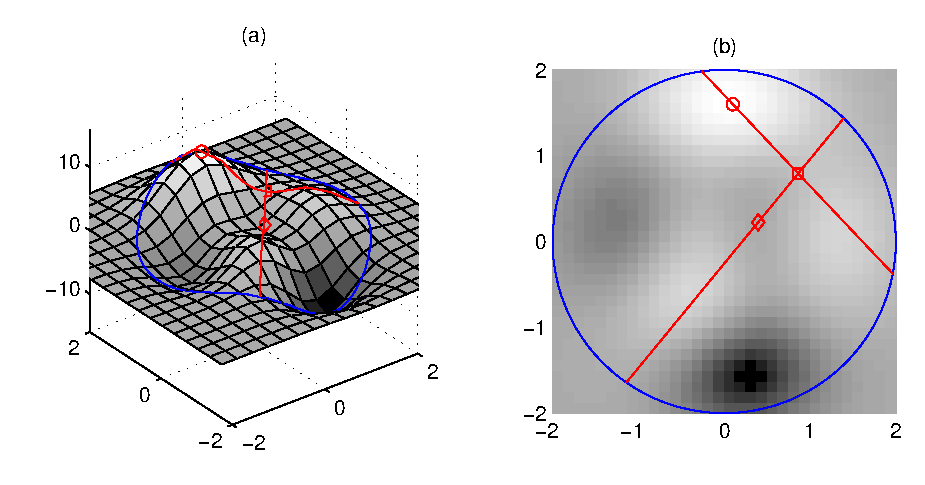
\includegraphics{figures/descent.epsg}
\end{center}
\begin{capt}{Schematic representation of gradient descent.}
Points within the blue circle are in \calF, the height of the surface
the value of (\ref{eqn:theory:cost function}) at that point.  (a) is a
3D view, (b) is top view. Red lines show line searches; markers
minimums.  Descent from $\circ$ to $\Box$ to $\Diamond$, where it
terminates due to local minimum.
\end{capt}
\label{fig:gradient descent}
\end{linefigure}

This statement is formalised in the following theorem.

\begin{theorem}[AdaBoost implements gradient descent]
The AdaBoost algorithm implements gradient descent over a cost functional
%
\begin{equation}
Q(F, \bfx, y) = \exp \{-y F(\bfx) \}
\end{equation}
%
\proof We outline a skeleton, ignoring initial conditions and the
stopping conditions.  We will show that, given a state at iteration
$t$, then boosting and gradient descent produce identical states at
iteration $t+1$.

Once we have chosen $f_{t+1}$, we need to choose $w_{t+1}$.  This is
chosen to minimise the cost functional along the line given by the
direction $f_{t+1}$.  We can write the value of this cost functional
as
%
\begin{equation}
C = \sum_{i=1}^{m} c \left( y_i F_t(\bfx_i) + y_i w_{t+1}
f_{t+1}(\bfx_i) \right)
\end{equation}
Substituting in $c(f(x)) = e^{-yf(x)}$, we obtain
%
\begin{equation}
C = \sum_{i=1}^{m} \exp \left\{ y_i F_t(\bfx_i) + y_i w_{t+1}
f_{t+1}(\bfx_i) \right\}
\end{equation}
%
Now we need to differentiate this expression with respect to
$w_{t+1}$.   This task is simplified considerably by noting that only
the second half of the exponential term is variable with $w_{t+1}$.
The result is that
%
\begin{eqnarray}{ll}
\label{eqn:differentiate}
\frac{\partial C}{\partial w_{t+1}} &
= & \sum_{i=1}^{m} \frac{\partial}{\partial w_{t+1}}
\exp \left\{ y_i F_t(\bfx_i) + y_i w_{t+1}
f_{t+1}(\bfx_i) \right\} \nonumber \\
& = & \sum_{i=1}^{m} y_i \exp \left\{ y_i F_t(\bfx_i) + y_i w_{t+1}
f_{t+1}(\bfx_i) \right\} 
\end{eqnarray}
%
From this result, we make several simplifications.  Noting that
%
\begin{equation}
y_i f_{t+1}(\bfx_i) = \left{ 
	\begin{array}{ll}
	1 &	\qquad \mbox{if $y_i = f_{t+1}(\bfx_i)$} \\
	-1 &	\qquad \mbox{if $y_i \neq f_{t+1}(\bfx_i)$}
	\end{array}
\right.
\end{equation}
%
and that $w_{i | t} = k \exp \{ -y_i F_t(x_i) \}$ where $k$ is some
constant, we can recast (\ref{eqn:differentiate}) into the form
%
\begin{equation}
\underbar{\frac{\sum_{i : y_i = f_{t+1}(\bfx_i)} w_{i|t}}
{\sum_{i : y_i = f_{t+1}(\bfx_i)} w_{i|t}}}{\epsilon_t} 
= \exp \( 2 \alpha \}
\end{equation}
%
from which it is a simple transformation to obtain
(\ref{eqn:theory:bt}).  Thus, the state at iteration $t+1$ is
equivalent to boosting; thus boosting implements gradient descent.
\end{theorem}

\subsection{Summary}



\section{Properties of the boosting algorithm}

* Guaranteed convergence to zero training error

  * It modifies the weights at each iteration so the previous had
    $\epsilon_t = 1/2$

  * So we must keep on getting better

  * So we must converge

* Scale invariance

  * The sign makes it not matter

  * If we multiply $F_t$ by $k$ to get $F*_t$, then we get $b*_{t+1} = 1/k
    b_{t+1}$

* Converges to the solution that has the minimum margin
	
\subsection{Convergence of boosting}

\begin{theorem}
Given a weaklearner $\mathcal{L}$ and a training set $S$,
then either:
\begin{enumerate}
\item	The boosting algorithm will terminate; or
\item	There exists an iteration $t_{zero}$ such that for all $t \geq
	t_{zero}$ the training error $\epsilon_t = 0$.
\end{enumerate}

\proof If for any training iteration $t$ we have $\epsilon_t > 1/2$ then the
boosting algorithm will terminate.  Assuming that this is not the
case, let us look at $\|b\|$.  As $t \rightarrow \infty$, $\|b\|
\rightarrow \infty$.  Thus, taking the normalised hypotheses $\bar{h}_i
= b_i \frac{h}{\sum b}$ we get the cost function as
\[
C(F_{t+1}) = \sum_{i=1}^{m} \exp\left\{ -y_i b_i h_i(x_i)
\right\}^{\|b\|}
\]
Now, we know from theorem (number?) that the boosting algorithm will
always find the global minimum of the cost function.  Since all $b_i >
0$, this is achieved when all training examples are classified
correctly...

Need a lot more work on this proof.  Do I want to show that since it
gets steeper and steeper, the cost of a negative sample gets too
large?  I don't think that the way I am doing it is going to work,
really.  I need to show that because
\begin{itemize}
\item	The weights for wrong samples are increasing exponentially,
	and
\item	The power that the cost function is raised to makes the wrong
	margin get worse and worse,
\end{itemize}
then the thingy gets minimised...

I need to bring the training error < 1/2 into it somewhere.  I think
that I can show that if
\begin{itemize}
\item	$\|b\|$ increases without bound; and
\item	$\epsilon_t$ is always < 1/2, then
\end{itemize}
I don't know!

\end{theorem}



\subsection{Size of $b$}

The following theorem shows that the total weight of the boosting
algorithm is unbounded as the number of iterations increases.  It is
used to prove results on the minimum margin and final training error
of boosting.

\begin{theorem}
The size of the $b$ weight vector, $\|b\| \rightarrow \infty$
as $t \rightarrow \infty$ (assuming the boosting algorithm doesn't
terminate).

\proof ?
\end{theorem}


\subsection{Minimum margin}

The following proof shows that the solution that AdaBoost converges to
is the one that maximises the minimum margin on the training samples.

\begin{theorem}
Given a particular learning algorithm $F$ and a training
set $S$, define the minimum margin as
\[
m_{\min} = min_{\{x,y\} \in S} y_i F(x_i)
\]
Then the boosting algorithm will converge as $t \rightarrow \infty$ to
the solution which maximised the minimum margin.

\proof For boosting we can write $F_t = b_1 f_1 + \cdots + b_t f_t$.
Then defining our \emph{normalised hypotheses} $\bar{f}_i$ as
\[
\bar{f} = \frac{b_i f_i}{\|b\|}
\]
such that $\hat{F}_t = \bar{f}_1 + \cdots + \bar{f}_t$, we can write
our cost function (reference?) as 
\[
C(b, S) = \sum_{i=1}^{m} \exp\{-y_i \bar{F}_t(x_i)\}^{\|b\|}
\]
We already know from the gradient descent theory (reference?) that we
are trying to minimise the cost function.  Now as $\|b\| \rightarrow
\infty$ (from the previous theorem) the largest value of $\exp\{-y_i
\bar{F}_t(x_i)\}$ will dominate, and so $C(b, S) \rightarrow exp\{\max
-y_i \bar{F}_t(x_i)\}$.  Thus, by minimising $C(b, S)$, we are making
$\min y_i \bar{F}_t(x_i)$ as large as possible; that is we are
maximising the minimum margin.
\end{theorem}


\subsection{Scale invariance of strong hypotheses}
\begin{theorem}
The hypothesis returned by the AdaBoost is independent of a linear
scaling of the $b$ values.  In particular, for all $k > 0$, the
scaled hypothesis $kF$ is equivalent to the unscaled hypothesis $F$.

\proof In order to prove this equivalence, we show that for any
training sample $\{x, y\}$ both $F$ and $kF$ return the same result.

(Proof continues noting that the sign function is independent of
scaling)
\end{theorem}

We denote this equivalence by writing
\[
kF \equiv F
\]


\subsection{Scale invariance of AdaBoost}

The following theorem takes the previous result one step further,
showing that is AdaBoost is given a scaled hypothesis $kF$ instead of
$F$, it will choose a $b$ value that is also scaled by the same
amount.

this is not true... look at Gunnar's notes again

\begin{theorem}
Assume a strong hypothesis $F_t(\cdot) = b_1 f_1(\cdot) + \cdots + b_m
f_m(\cdot)$.  Denote the training action of the AdaBoost algorithm as
$F_t(\cdot) \Rightarrow F_{t+1}(\cdot) = F_t(\cdot) +
b_{t+1}f_{t+1}(\cdot)$.  If
\[
	F_t(\cdot) \Rightarrow F_t(\cdot) + b_{t+1}f_{t+1}(\cdot)
\]
then
\[
	kF_t(\cdot) \Rightarrow k\left( F_t(\cdot) +
	b_{t+1}f_{t+1}(\cdot) \right)
\]
and thus
\[
	kF_{t+1} \equiv F_{t+1}
\]

\proof We show that the minimum of the cost function occurs at
$kb_{t+1}$ instead of $b_{t+1}$.
\end{theorem}



These are from \cite{Ratsch98}:

\begin{theorem}[Weight update of AdaBoost (Schapire \cite{Schapire97})]
The weights $w_{i|t}$ in the $t$-th iteration are chosen such that the
previous hypothesis has exactly a weighted training error $\epsilon$
of $1/2$.
\end{theorem}

\subsection{Summary}


\section{Performance bounds for Boosting}
By proceeding I mean somewhere in Peter's book chapter

I need to rewrite this section; it is copied verbatim

The preceding ideas can be applied to the boosting algorithm.  Let us
take in particular the boosted classifier of the form
\begin{equation}
x \mapsto \sign \left( \sum_{i=1}^{N} w_i f_i(x) \right)
\end{equation}
that have large margins on the training examples, where $w_i > 0$,
$\sum_i w_i = 1$, and $f_i$ are classifiers in some class $H$.  A
VC-dimension analysis would suggest that the generalisation error
would of these classifiers would increase with $N$, the number of base
hypotheses $f_i$ that are combined.  The following result, which
follows easily from techniques developed in \cite{Bartlett98}, shows
that the fat-shattering dimension of the class of convex combinations
of classifiers is independent of the number of base hypotheses.

\subsection{Bounds on fat-shattering dimension in boosting}

* Can't state this directly.  Substitute in the bound on covering
  numbers from eg. Peter's slides, and state that instead.

There is a constant $c$ so that for all classes $H$ of functions
mapping from $X$ to $\{-1, 1\}$, the class of convex combinations of
functions from $H$ satisfies
\begin{equation}
\fat_{\calF} \leq c \frac{h}{\gamma^2} \ln (1/\gamma)
\end{equation}

where $h$ is the VC-dimension of the class $H$ of base hypotheses.

\subsection{Bounds on error in boosting}

* Again, make use of the covering numbers result from last time,
  substitute in to get this.  If substituting directly gives a better
  bound, then use that.

There is a constant $c$ such that, for the class \calF\ of convex
combinations of classifiers from a class $H$ with VC-dimension $h$,
for all probability distributions, with probability at least
$1-\delta$ over $l$ independently generated training examples, every
classifier $\sign(f) \in \sign(\calF)$ has error no more than
\begin{equation}
b/l + \sqrt{\frac{c}{l} \left[ \frac{h \ln^2 (l/h)}{\gamma^2} +
\ln(1/\gamma) \right] }
\end{equation}
where $b$ is the number of labelled training examples with margin less
that $\gamma$.

\subsection{Summary}

\section{Overfitting}


\section{Normed boosting algorithms}


\section{Chapter summary}



